
\documentclass[progress]{cmpreport}
\usepackage{hyperref}
\newcommand{\head}[1]{\textnormal{\textbf{#1}}} %Used for tables
\usepackage{fontenc}  % \textsterling for £
\usepackage{caption}

\title{Designing, Building, Coding and Tracking a Mechanical Hand/Arm}
\author{Deborah Taylor}
\registration{100085169}

\supervisor{Dr Graeme Richards}
\date{\today}
\ccode{CMP-6013Y}

\summary{Draft as of \today.}
\acknowledgements{}

% If the figures do not fit on one page, comment this line out
\onePageLists
%\linespread{1.5}
\bibliographystyle{apalike} 

% Prevents author/year errors
\usepackage{natbib}
\usepackage{float}
\usepackage{rotating}
\usepackage[strings]{underscore}
\usepackage{wrapfig}
\usepackage{graphicx} 
\usepackage{subcaption} %  for subfigures environments
\usepackage[nopar]{lipsum} 

\begin {document}


\section{Introduction}
The first commercial arm was designed in 1954, by George C. Devol\footnote{George Charles Devol, Jr. American Inventor born 20 Feb 1912 and died 11 Aug 2011} and this used a claw to grip items.

\begin{wrapfigure}{L}{0.5\textwidth}
	\caption{Commercial Claw/Arm Example} 
	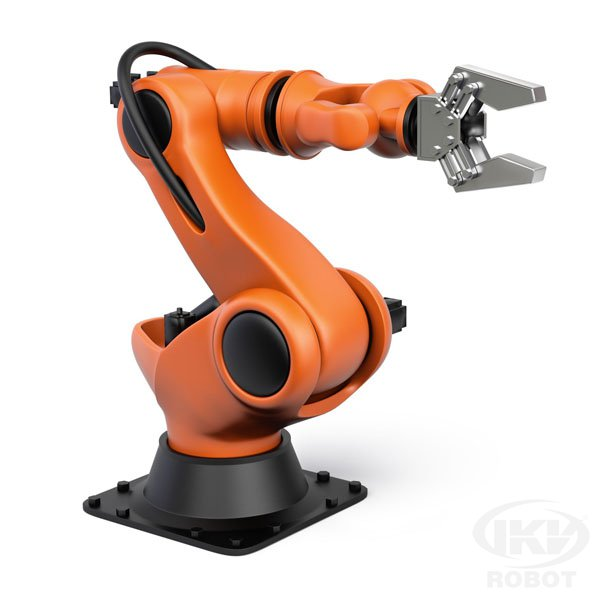
\includegraphics[width=0.7\linewidth]{photos/claw.jpg}  
\end{wrapfigure}
Robotics have advanced considerably since then, however, commercial arms continue to be built using claws and this stops them being very dexterous or flexible (see figure 1)\footnote{Source for figure 1: https://www.alibaba.com/product-detail/6-axis-industrial-robot-industrial-robot_60498256063.html}. It also makes them more likely to fail if the claws are not aligned correctly, or one stops working. \citep{devol}, \citep{grigorediscovering}.  

To increase manoeuvrability and flexibility the mechanical arm needs to be redesigned so it can replicate a normal human hand. 

The purpose of this project is to build a bespoke mechanical hand/arm that will use fingers to pick up and put down items and a sensor or camera to track items or movement. This will enable the project to develop a flexible hand that will continue to work, even if one of the fingers is broken or not in alignment. 


\section{Motivation and Aims}

\textbf{\underline{Motivation:}} Prosthetics has been an interest, ever since the author's school friend developed meningitis at an early age and ended up losing an arm. The author saw how difficult it was for that person to complete even the simplest task, such as dressing or tying a shoelace. 

With current skill levels and the project time-frame, it is not feasible to develop a fully functioning prosthetic limb, therefore, the author has shifted focus to commercial uses instead. Commercial arms are more straight forward to develop and are used in a multitude of industries from manufacturing to defusing bombs. 

This project will enable the author to develop their skills, while still producing a product that can be used in a commercial marketplace. 

If the project were to continue, into a future development stage, the hardware could be adapted for use in health research and prosthetics. \newline

\noindent\textbf{\underline{Aims:}} The project's aim, as mentioned in the introduction, is to design and build a mechanical hand/arm, with coding to fully demonstrate flexibility and functionality of a human hand. 

The hardware will be able to complete basic tasks such as moving each finger, moving the hand/arm up, down, left and right, plus, picking up and putting down an item. It will, also, have more complex coding to play Rock, Paper, Scissors\footnote{Played between two people. Each player forms one of three shapes with an outstretched hand. "Rock" is a closed fist, "Paper" is a flat hand and "Scissors" is a fist with the index and middle fingers extended. It has only two outcomes, either a tie or one of the players win.} or solve the Towers of Hanoi\footnote{Object of the game is to move all the disks over to Tower 3 but you cannot place a larger disk onto a smaller disk} \citep{DBLP:conf/case/ItoSYI16}, \citep{DBLP:journals/corr/abs-cs-0612070}.  

The author is currently investigating which of these is best for the project, so the design and build is being processed so either can be selected.

If Rock Paper Scissors is chosen this will show the full flexibility of the hand and the tracking will involve identifying when a person is ready to play.

If the Towers of Hanoi is chosen this will use tracking to identify items and the hand will pick up and move them to different places.

Whichever option is selected, any movement specific to the other, will be incorporated into the basic coding to ensure full flexibility is demonstrated. 


\section{Design and Hardware Build}

An online Trello board has been created to log each task, throughout the life of the project. This enables the author to continually monitor progress. To view this Trello board access: https://trello.com/b/cdHgyGX0.

As this project involves both hardware and software a Software Engineering Design Document is needed to show designs, development and testing\footnote{A Design Document is a technical guide for Developers and includes Definitions, Requirements, Use Cases, etc.}. The author believes this is the most efficient way (in association with the Trello board) to ensure each stage of the design and build is completed in the correct order \citep{mcelrath}. \newline

\noindent{\textbf{\underline{\LARGE{D}{\large{esign:}}}} \newline

\noindent{The full Design Document is too large to include in this report, so an overview is covered here.}

\subsection{Similar Systems Analysis}
One of the first stages in designing any hardware and software is to investigate and review similar products, to see which features are available and how they differ from the new one being designed. 

This ensures there is no crossover of hardware or software already in existence and helps clarify specifications, requirements and scope. This can help identify if any "off the shelf" hardware or software is available and, if not, whether there is anything that can be adapted for the new project.

See figure 2 below for analysis of five mechanical arms already in use:

\begin{figure}[H] 
	\caption{Analysis of 5 different mechanical arms}
	\centering
	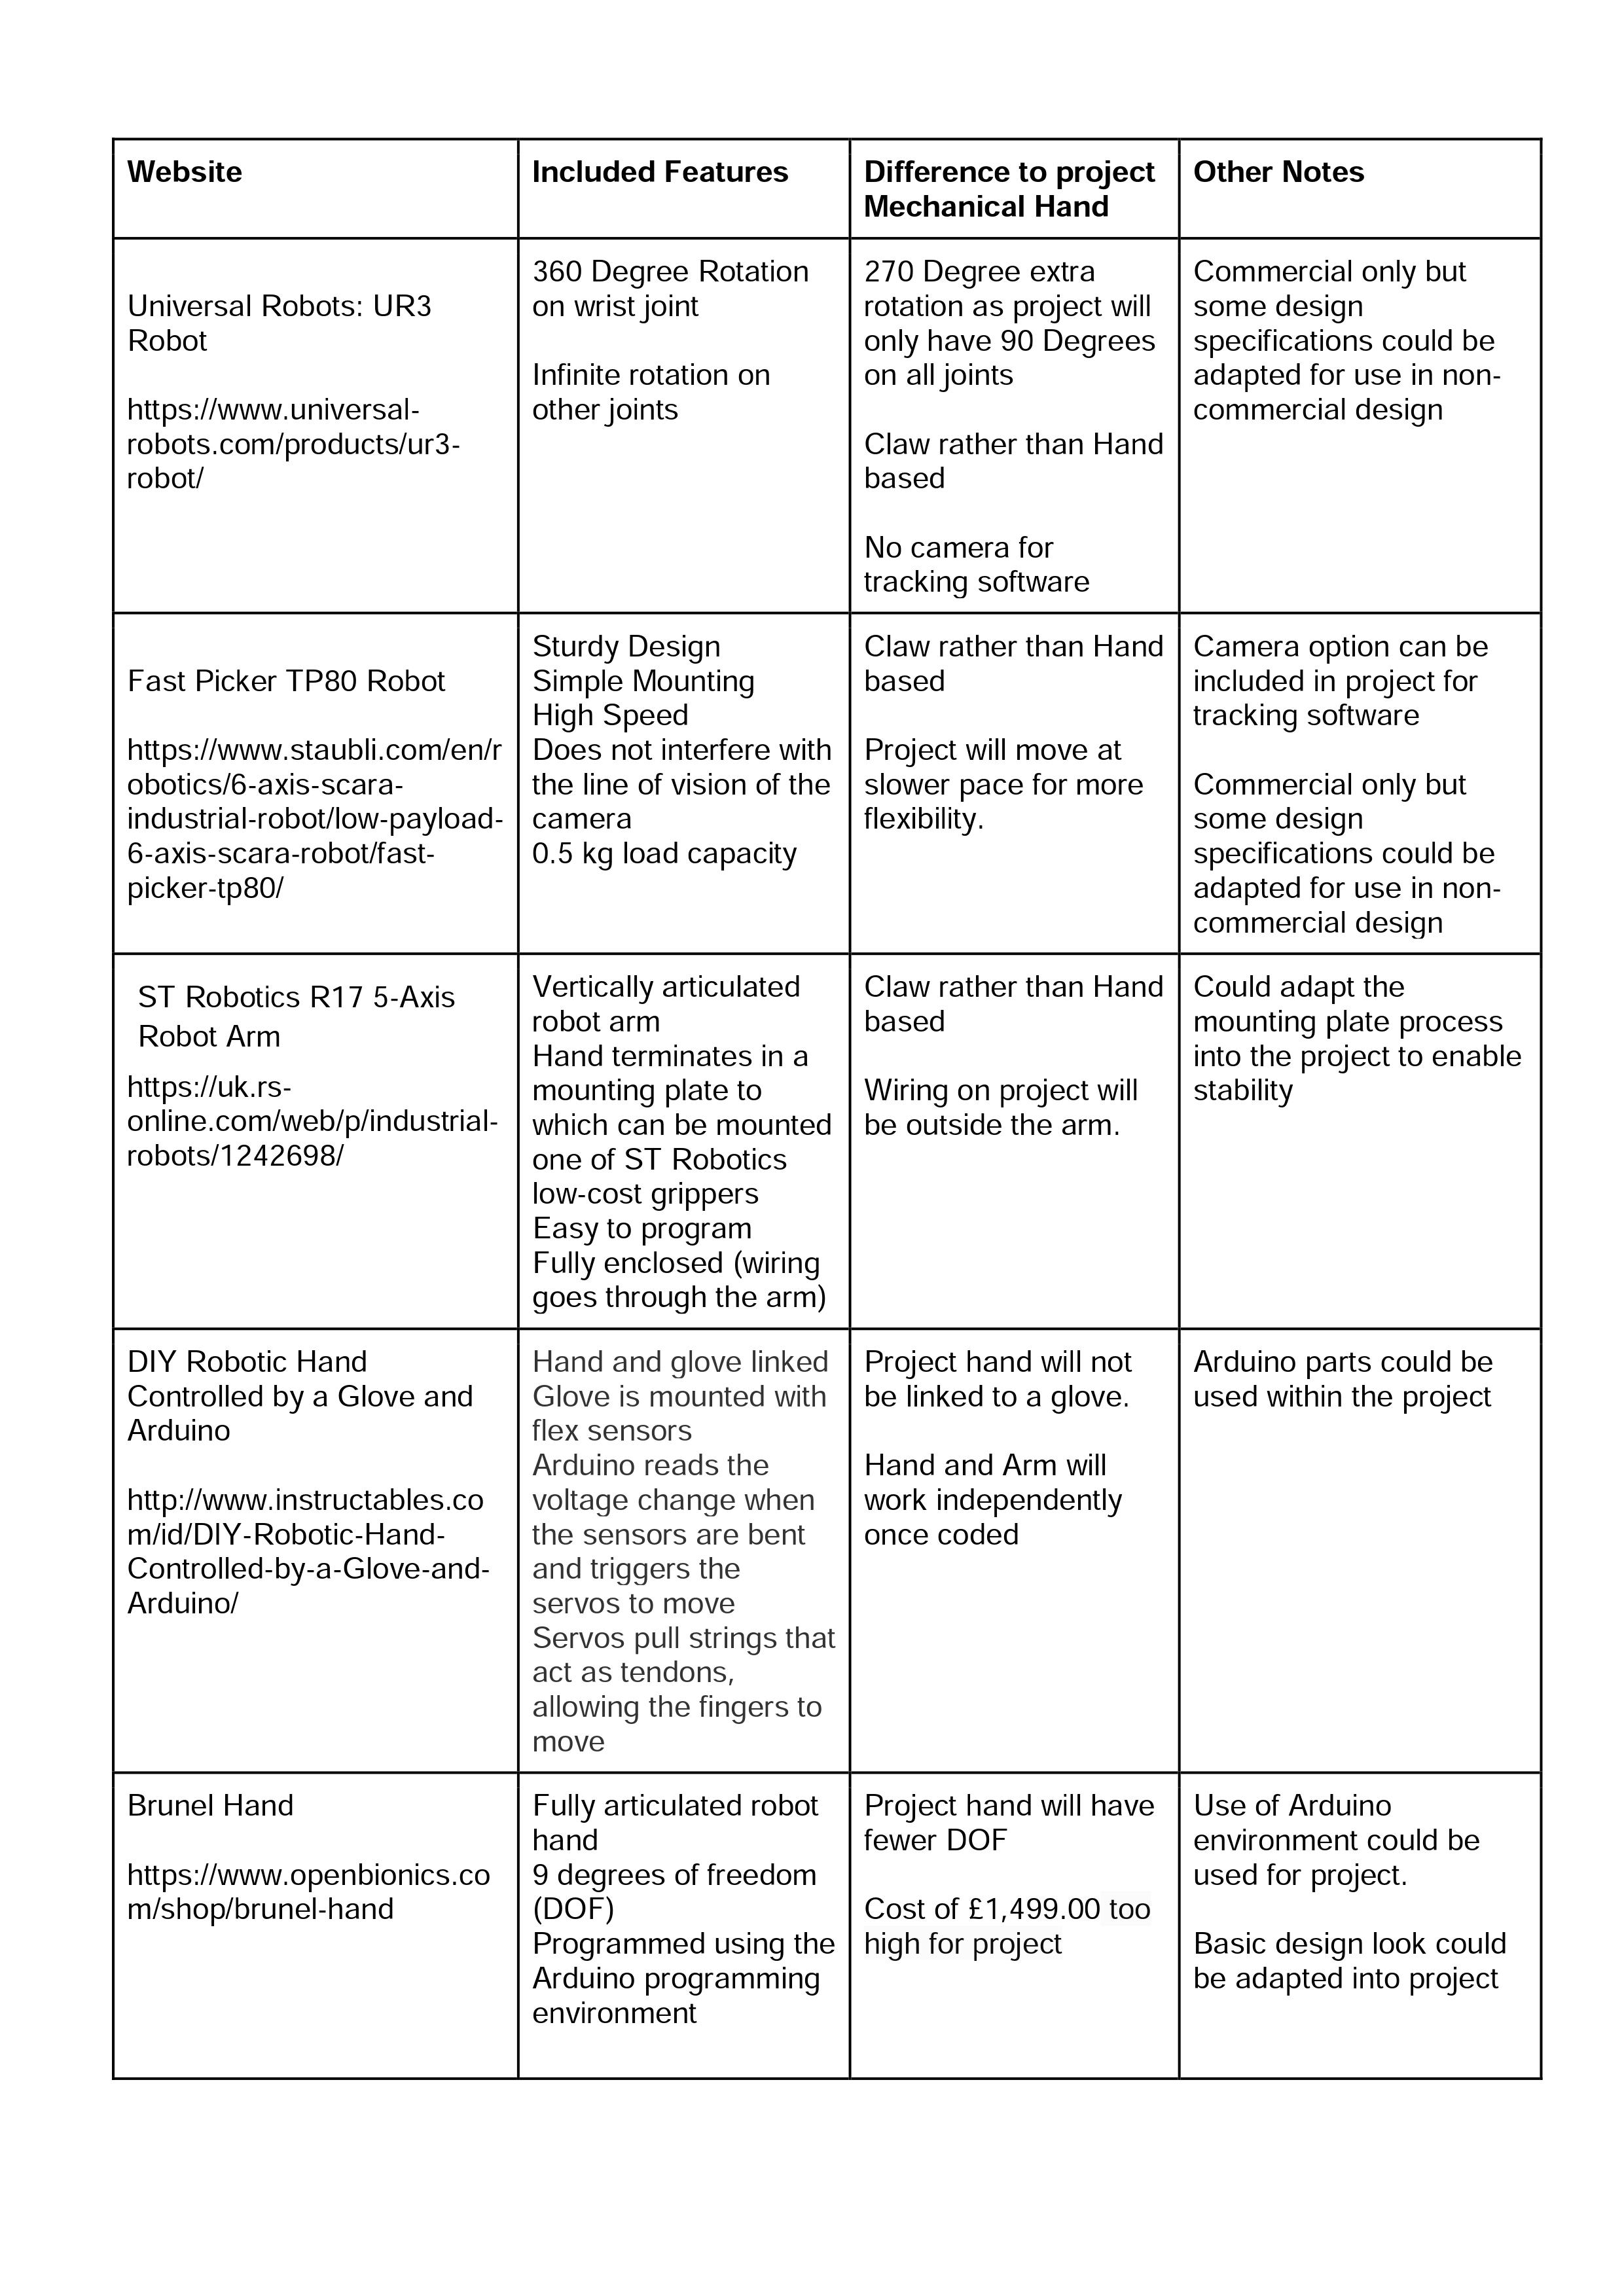
\includegraphics[trim=0cm 2.8cm 0cm 0.15cm, width=1 \textwidth, height=0.7 \textheight]{photos/SSA.jpg}
\end{figure}

\subsection{MoSCoW Analysis:}
Once the \textit{Similar Systems Analysis} is completed the next stage is the \textit{MoSCoW Analysis}.

This process determines the different requirements that will be in and out of scope for the project, along with priority levels for development. 

This analysis is made up of \textit{Must Have, Should Have, Could Have} and \textit{Won't Have} tasks. \newline

\noindent{\textbf{{Must Have:}}
These tasks are identified as absolutely crucial, at base level, for the project to work. They are prioritised within development and the \textit{Should Have} section will not be started until these are fully completed and tested. 

\begin{itemize}
	\item \textit{Skeletal hand design and arm (up to the equivalent of an elbow)}
	\item \textit{Fingers and thumb that can move independently and/or together}
	\item \textit{Movement rotation of 90 degrees, up, down, left and right}
	\item \textit{Basic coding to enable movement of the arm: up, down, left and right}
	\item \textit{Basic coding to enable the hand to pick up, hold and put down an item} %\newline
\end{itemize} 

\noindent{\textbf{{Should Have:}} 
These tasks are identified as necessary to the project to increase effectiveness within the design. They are the second stage of a development and will only be started, once the \textit{Must Have} tasks are completed.
\begin{itemize}	
	\item \textit{Complex coding to enable hardware to play Rock, Paper, Scissors or solve Towers of Hanoi puzzle}
	\item \textit{Sensor or Camera connected to the hardware (with or without a wire) to identify items or movement} %newline
\end{itemize}	

\noindent{\textbf{{Could Have:}}
These tasks are identified as nice to have, but not necessary for the project to be successful. These are desired and may be implemented, depending on cost and the time-frame available. 
\begin{itemize}	
	\item \textit{Ability to move independently of a PC or laptop (utilising a servo controller mounted on the arm)}
	\item \textit{Haptic sensors to enable feedback on how the hand grips an item} %newline
\end{itemize}

\noindent{\textbf{{Won't Have:}} 
These tasks are identified as out of scope for the project and will not be implemented. If the project were to continue, into a future development stage, these could be implemented then.  
\begin{itemize}		
	\item \textit{Independent thought and movement eg Artificial Intelligence } 
\end{itemize}

\subsection{Use Case (UML) Diagram:}

Once the \textit{MoSCoW} analysis is completed a \textit{Use Case (UML) Diagram}\footnote{Unified Modelling language (UML) is a standard modelling language for developers to visualize and document tasks} is designed to show User interaction with the hardware \citep{AljamaanLBGF14}. From the above \textit{MoSCoW Analysis} the priorities identified, to show full hand flexibility and play either Rock, Paper, Scissors or solve the Towers of Hanoi, are:
\begin{itemize}		
	\item \textit{Move hand/arm up, down, left, right and open, close the hand}
	\item \textit{Move fingers independently and/or together so items can be picked up and put down}
	\item \textit{Use a sensor or camera to track movement and/or items}
\end{itemize}

As these priorities are necessary to the project, they need to be added to the \textit{Use Case UML Diagram}, to show how they interact and link together. See figure 3. 

\begin{figure}[H] 
	\caption{Use Case UML Diagram }
	\centering
	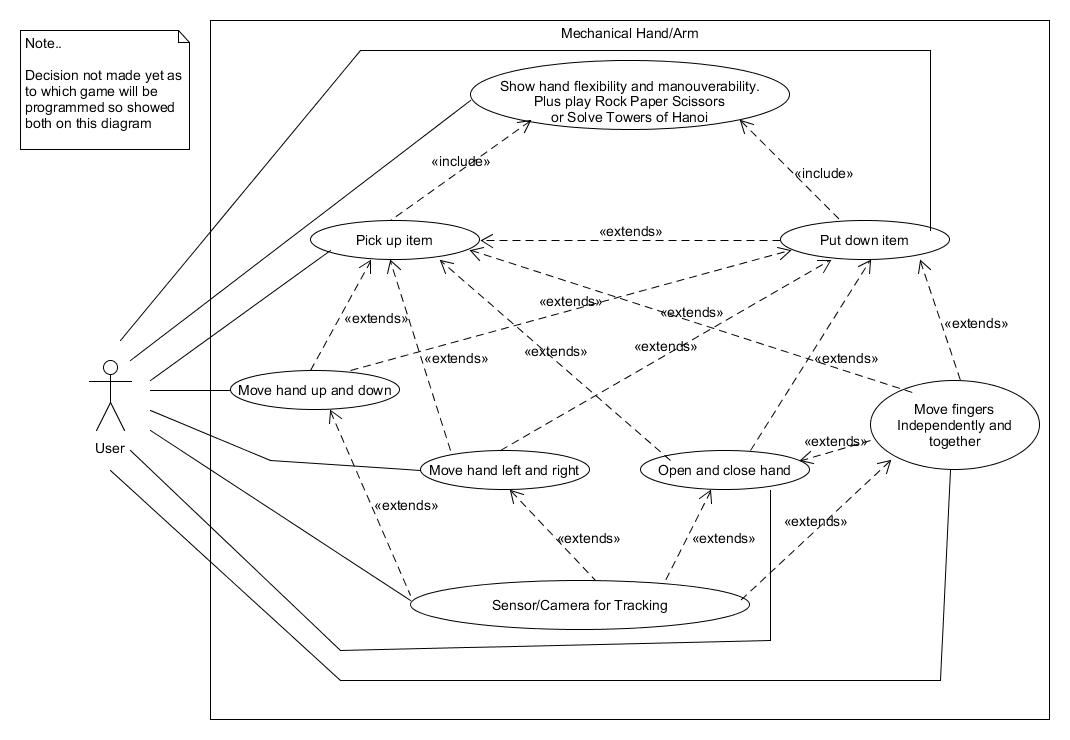
\includegraphics[width=0.7 \textheight]{photos/UMLdiagram.jpg}
\end{figure}

\subsection{Use Case Descriptions:}

Following completion of the \textit{Use Case UML Diagram}, \textit{Use Case Descriptions} are written, for each of the tasks shown on the diagram. See below for an example:
\begin{itemize}		
	\item \textit{Use Case 3 Open Hand: describes the process of connecting the laptop signal to the Hand hardware and enabling the Hand to open. This is a basic command that will be fundamental to the Hand movement for later, more complex, coding.}
\end{itemize}

\subsection{Detailed Use Case:}

The descriptions are then expanded into \textit{Detailed Use Cases}. These show steps required to achieve each task eg triggers, frequency, release schedules and provide information needed for development. See figure 4 below for an example:
\begin{figure}[H] 
	\caption{Use Case3: Open Hand Example}
	\centering
	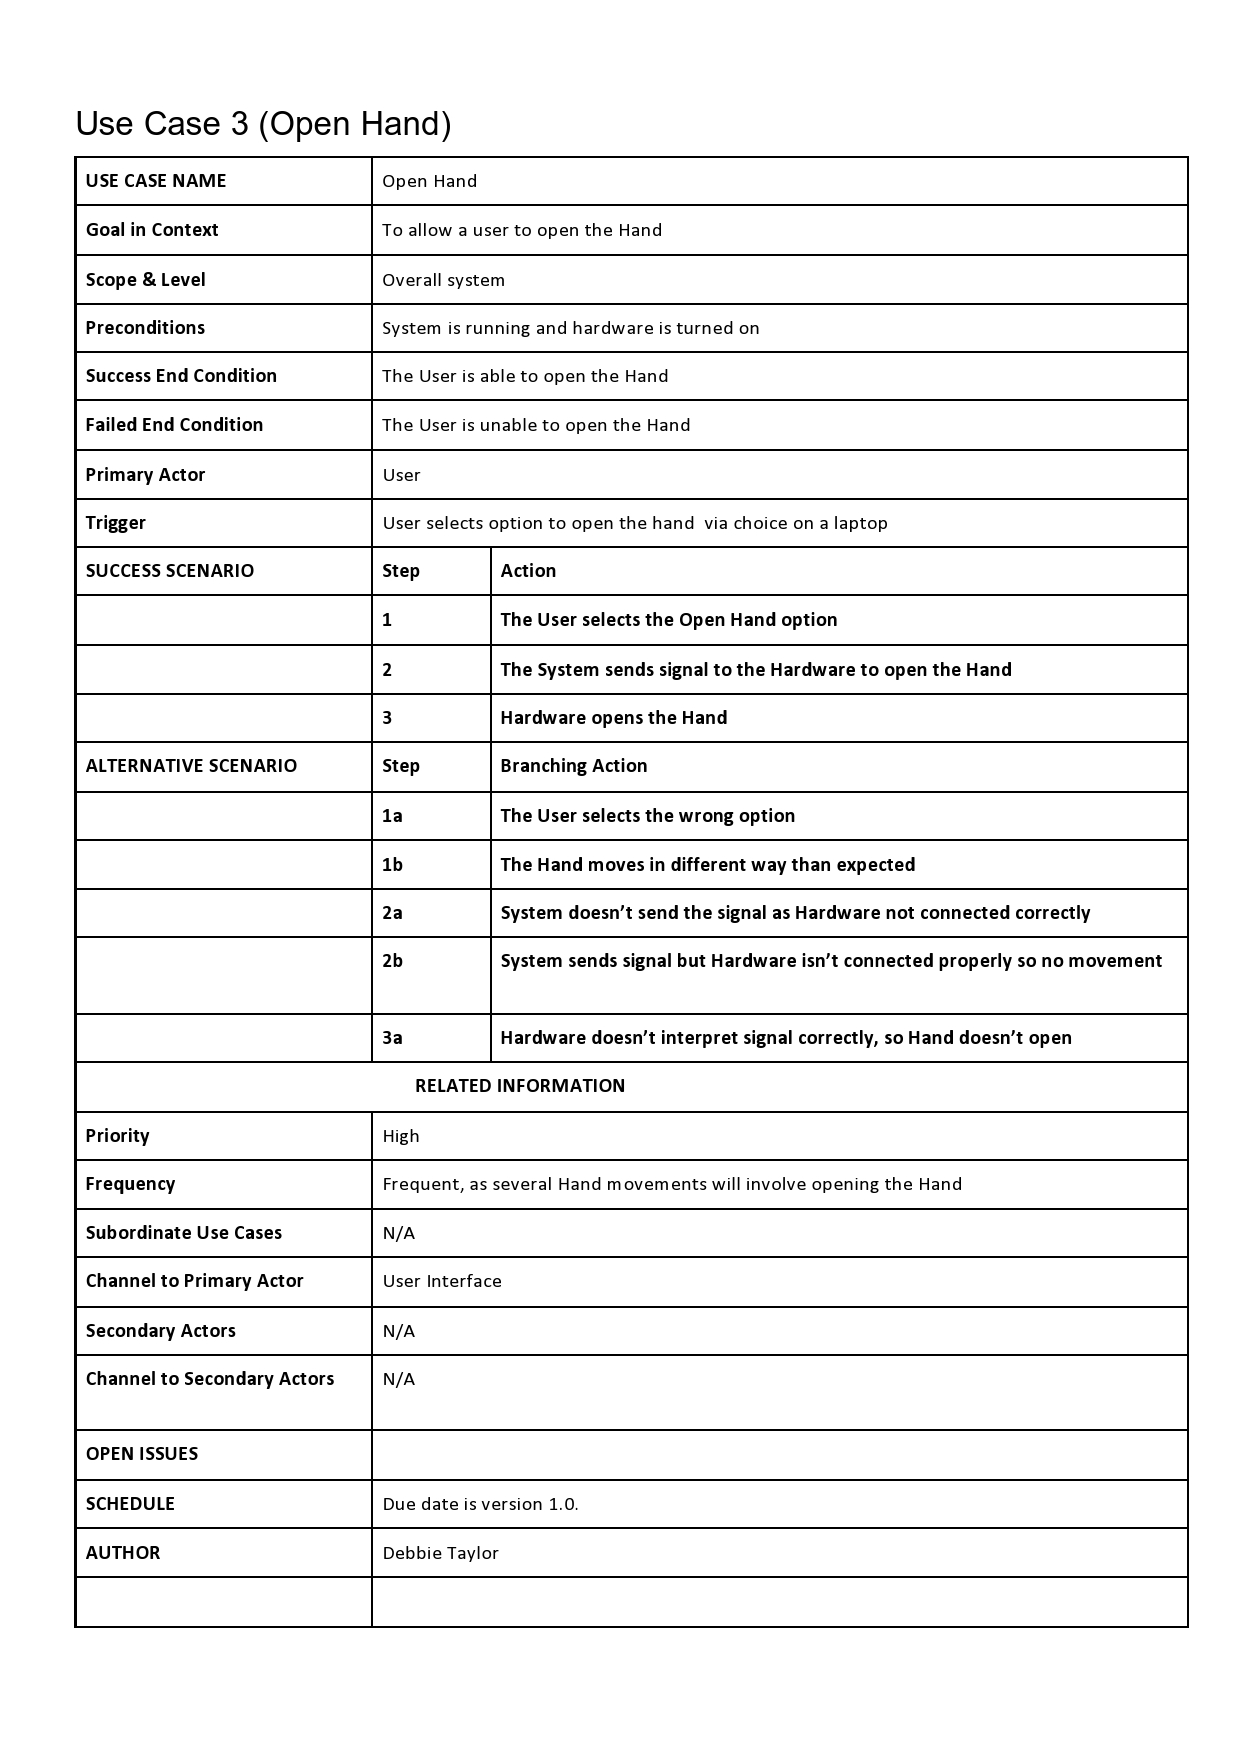
\includegraphics[trim=0cm 7cm 0cm 0.63cm, width=1.0 \textwidth, height=0.625 \textheight]{photos/UseCase_OpenHand.jpg}
\end{figure}

\subsection{Sequence Diagram:}

Once the \textit{Detailed Use Cases} are completed the final stage\footnote{As this is a hardware and software design there is no need for Architecture diagrams} is to create \textit{Sequence Diagrams}. These show step by step representations of specific scenarios. See figure 5 below for an example: 
\begin{figure}[H] 
	\caption{Sequence Diagram Example }
	\centering
	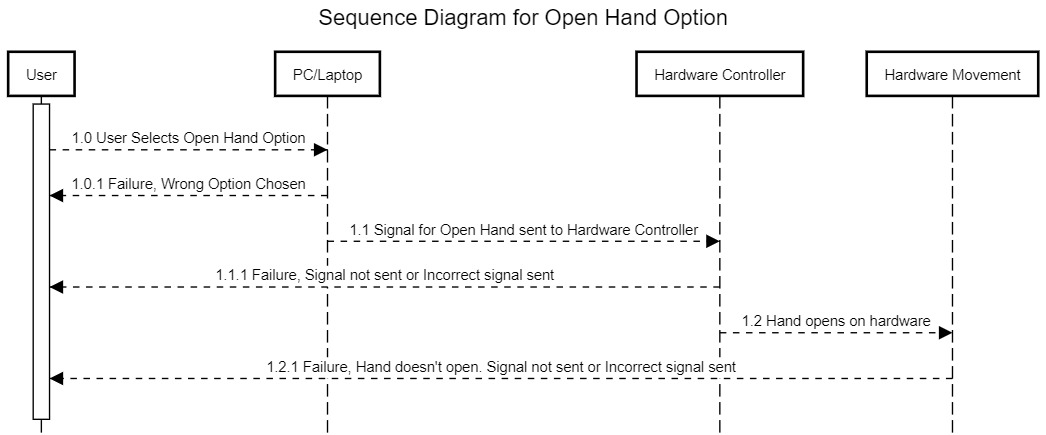
\includegraphics[ width=1 \textwidth]{photos/sequence_diagram.jpg}
\end{figure}

Completing this Design Document confirms there is no "off the shelf" skeletal hand/arm hardware available, so a bespoke build is required for this project. \newline 

\noindent{\textbf{\underline{\LARGE{H}{\large{ardware Build:}}}} \newline

\noindent{The Design Document also helps the author understand that a human hand is very complex.  In order for it to open, close, move each finger, hold items etc, a combination of the fingers, thumb and joints need work together.}

The first stage of the build, therefore, involves fully identifying how a human hand moves and what parts are needed to build the hardware.
\subsection{Skeletal Human Hand Investigation:}
\begin{wrapfigure}{L}{0.5\textwidth}
	\caption{Human Hand} 
	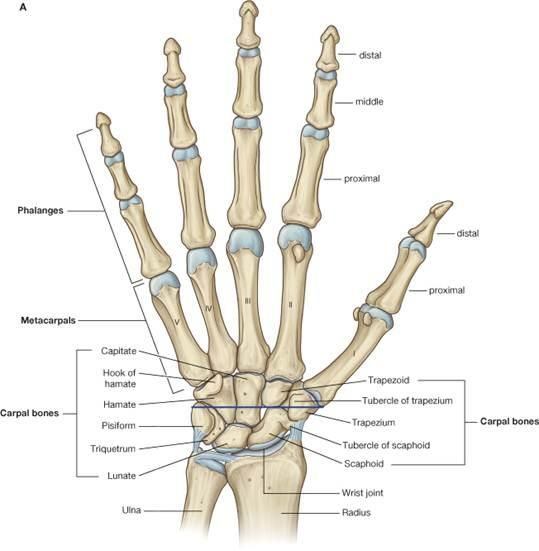
\includegraphics[width=0.7\linewidth]{photos/hand.jpg}  
\end{wrapfigure}

Due to the complexity mentioned above, the author needs to investigate the skeletal structure, by reading up on human anatomy and learning the names and connections for each part of a hand \citep{freivalds2011biomechanics}.

This identifies exactly which metal shapes need to be cut and how many servos, joints etc are needed to build the hardware. \newline

A friend (who is a machinist) supplies the bespoke metal skeleton "bone" parts for hand, using figure 6\footnote {Figure 6 Source: http://visual.merriam-webster.com/human-being/anatomy/skeleton/hand.php} as a template. They also provide the metal for use in the base and the arm.
 
The rest of the parts (servos, wiring, sensors, servo controller unit, ball-bearings etc) are obtained separately "off the shelf", using some of the ideas obtained from the \textit{Similar Systems Analysis}. 

The author originally decides to keep the build specific to a single brand name (eg Arduino) but a more cost effective approach is found while researching the skeletal structure. This involves buying "mix and match" parts from several different manufacturers, that can then be linked together on the hardware. 

\subsection{Hardware Build Progress:}

Due to the hardware being fundamental to the project, the build starts during the summer holidays and continues until the middle of Semester 1. Multiple photographs are taken showing step by step progress. 

See figures 7 to 10 below, for a selection of photographs showing build progression: 
\begin{figure}[H]
	\centering
	\begin{minipage}{0.455\textwidth}
		\caption{Start}
		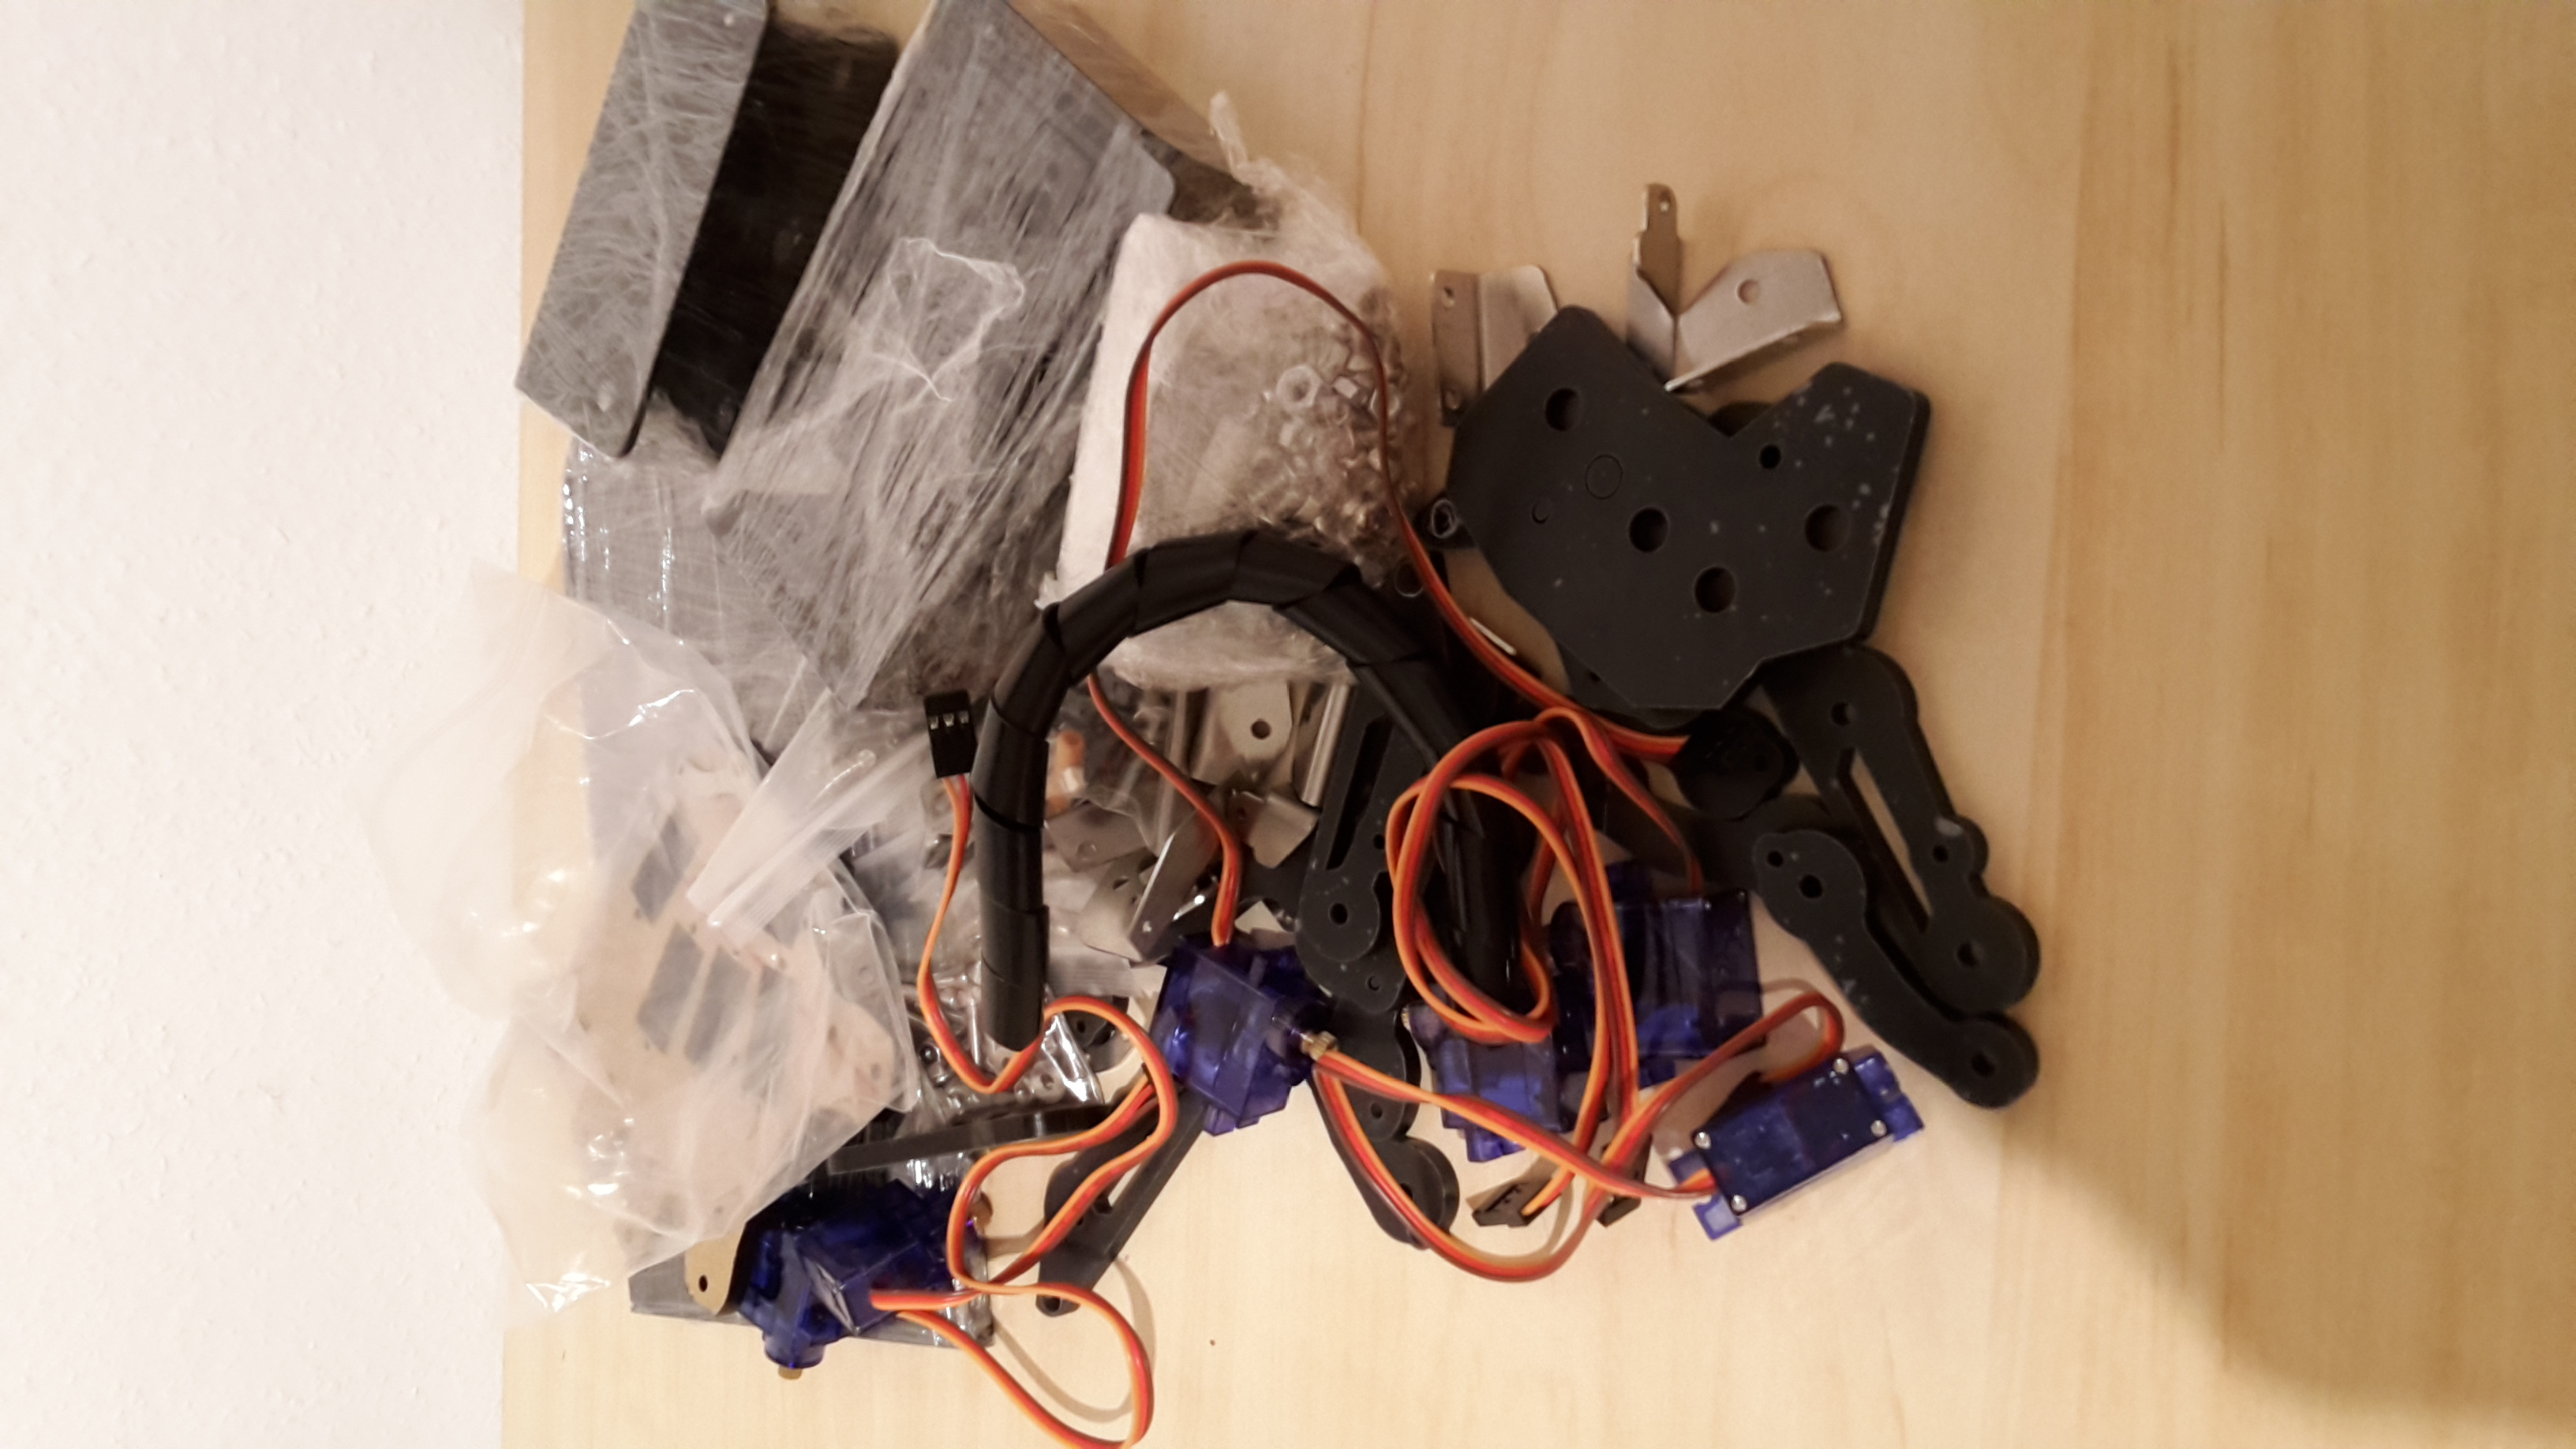
\includegraphics[width=1\textwidth, angle=-90]{photos/start.jpg}
	\end{minipage}
	\hfill
	\begin{minipage}{0.455\textwidth}
		\caption{Hand Built}
		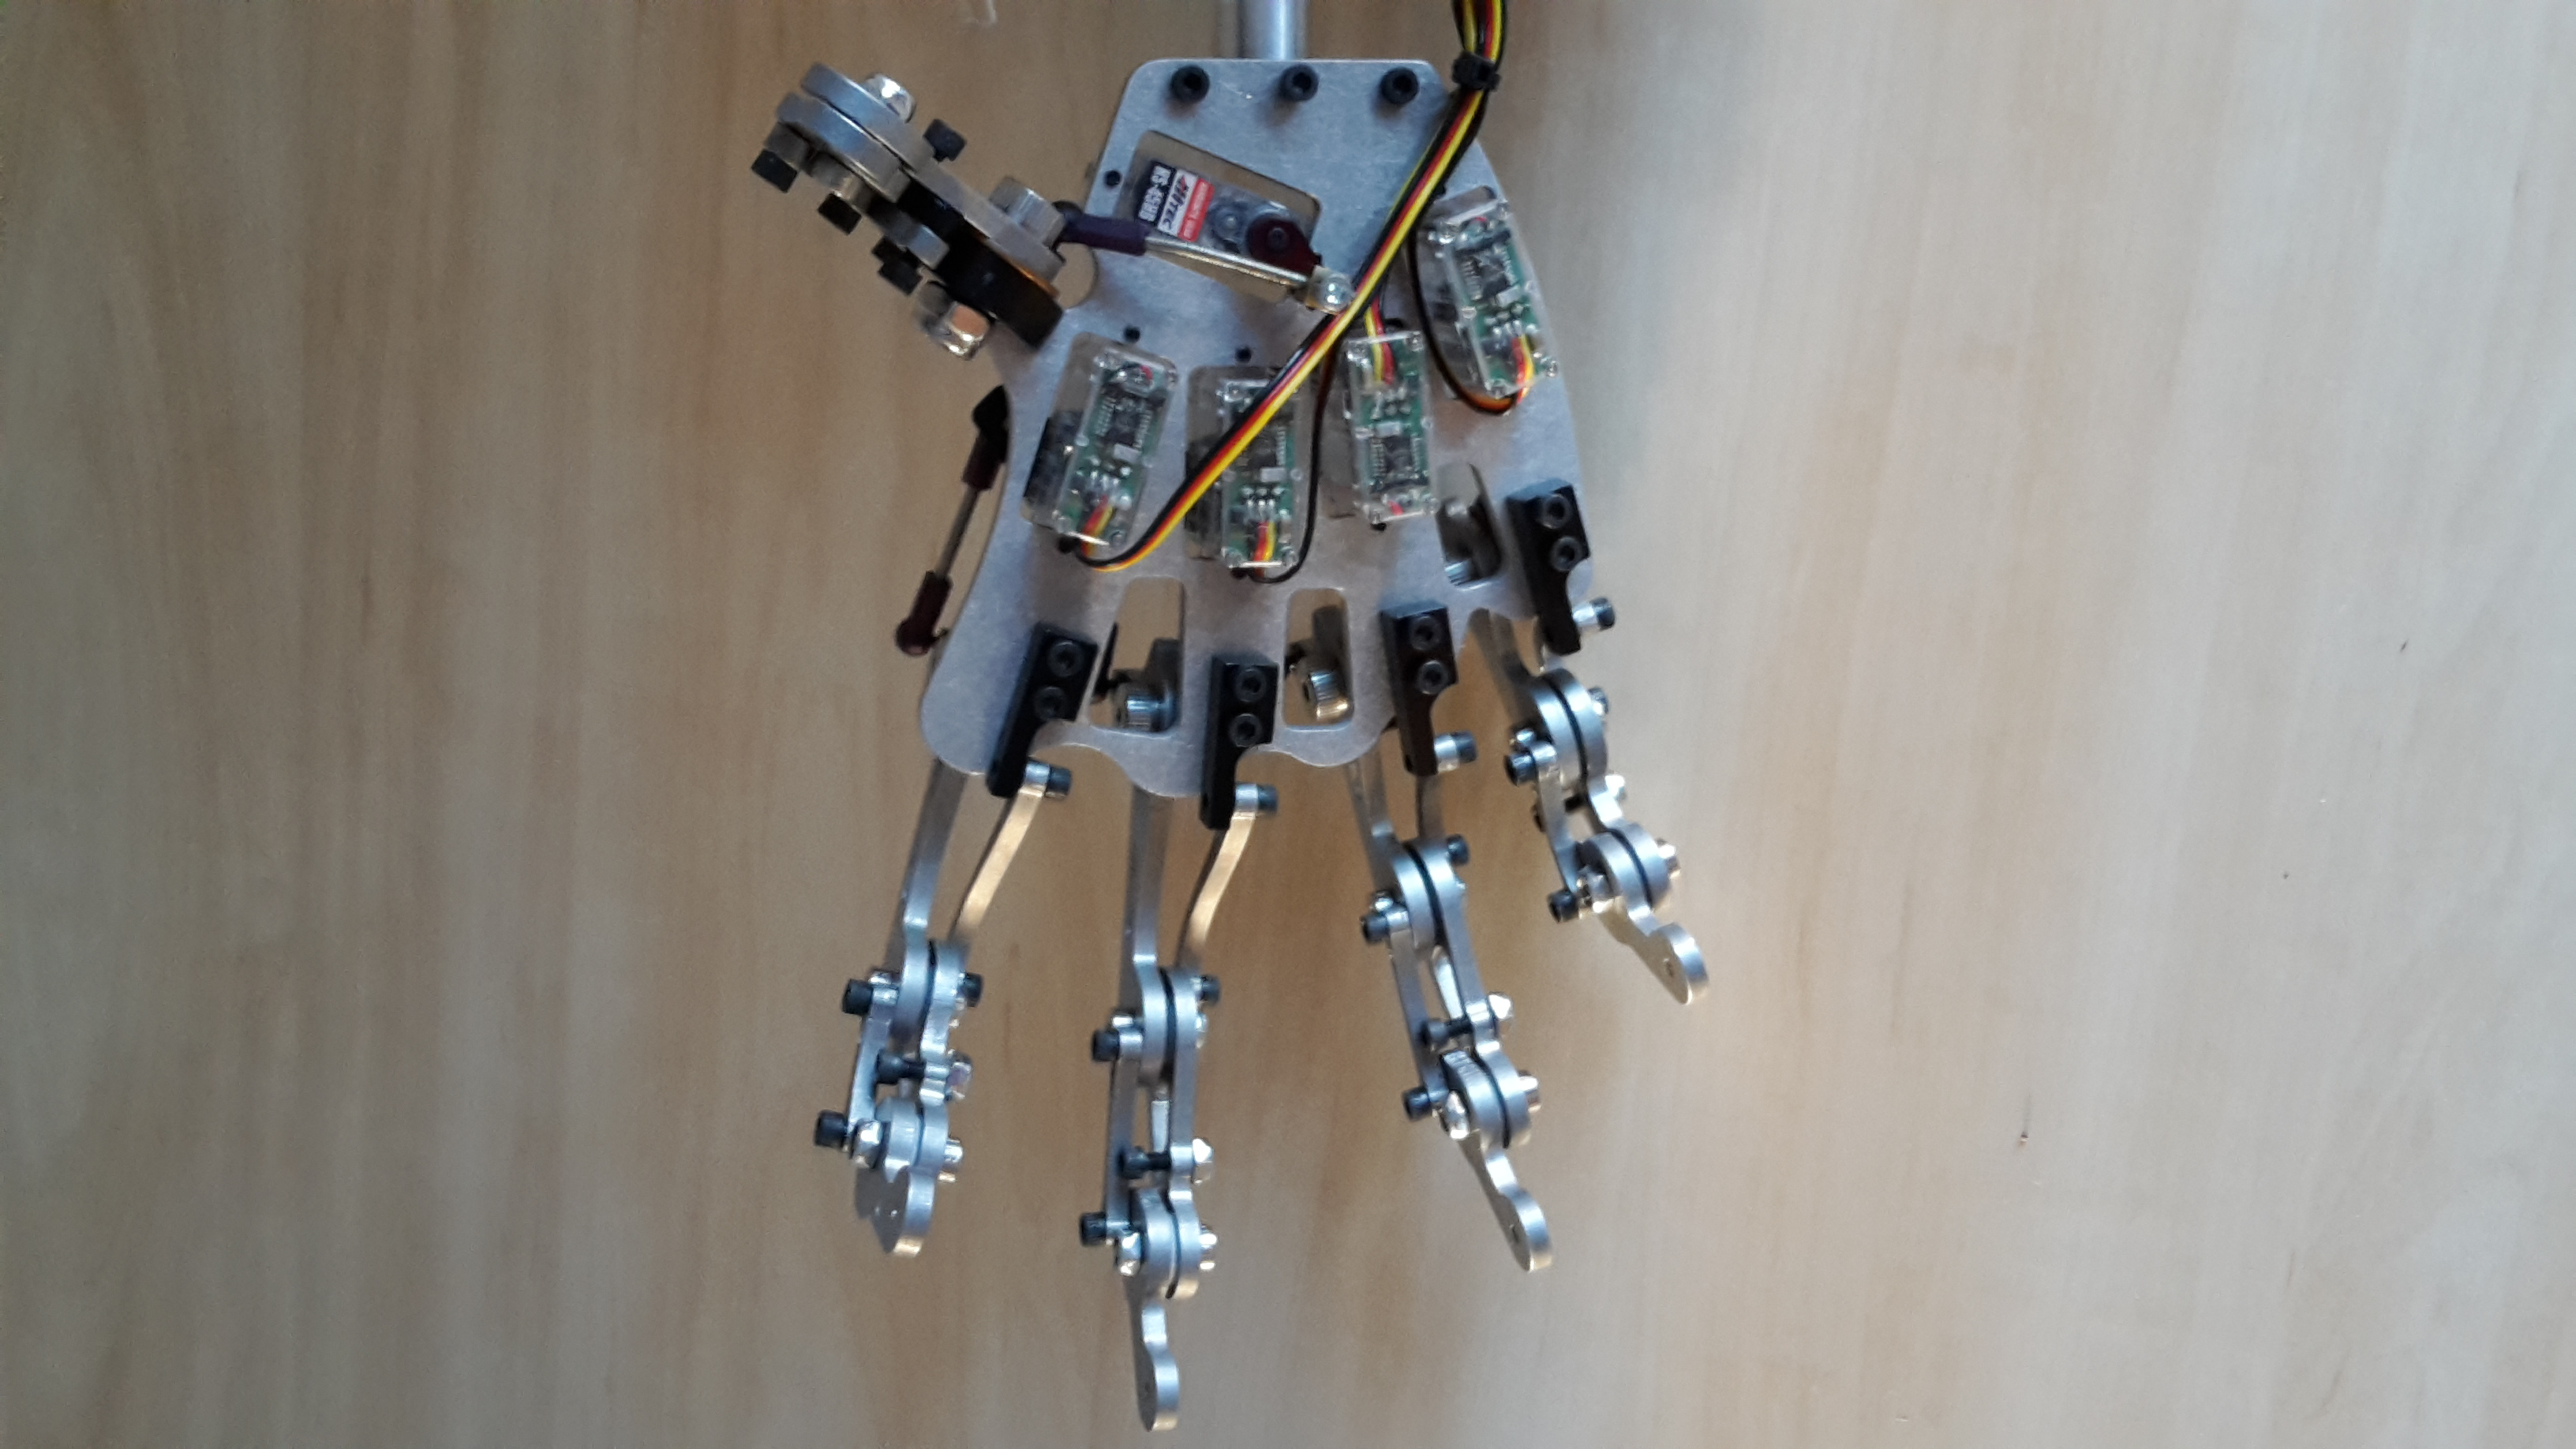
\includegraphics[width=1\textwidth, angle=-90]{photos/Day10.jpg}
	\end{minipage}
\end{figure}

\begin{figure}[H]
	\centering
	\begin{minipage}{0.455\textwidth}
		\caption{Arm Built}
		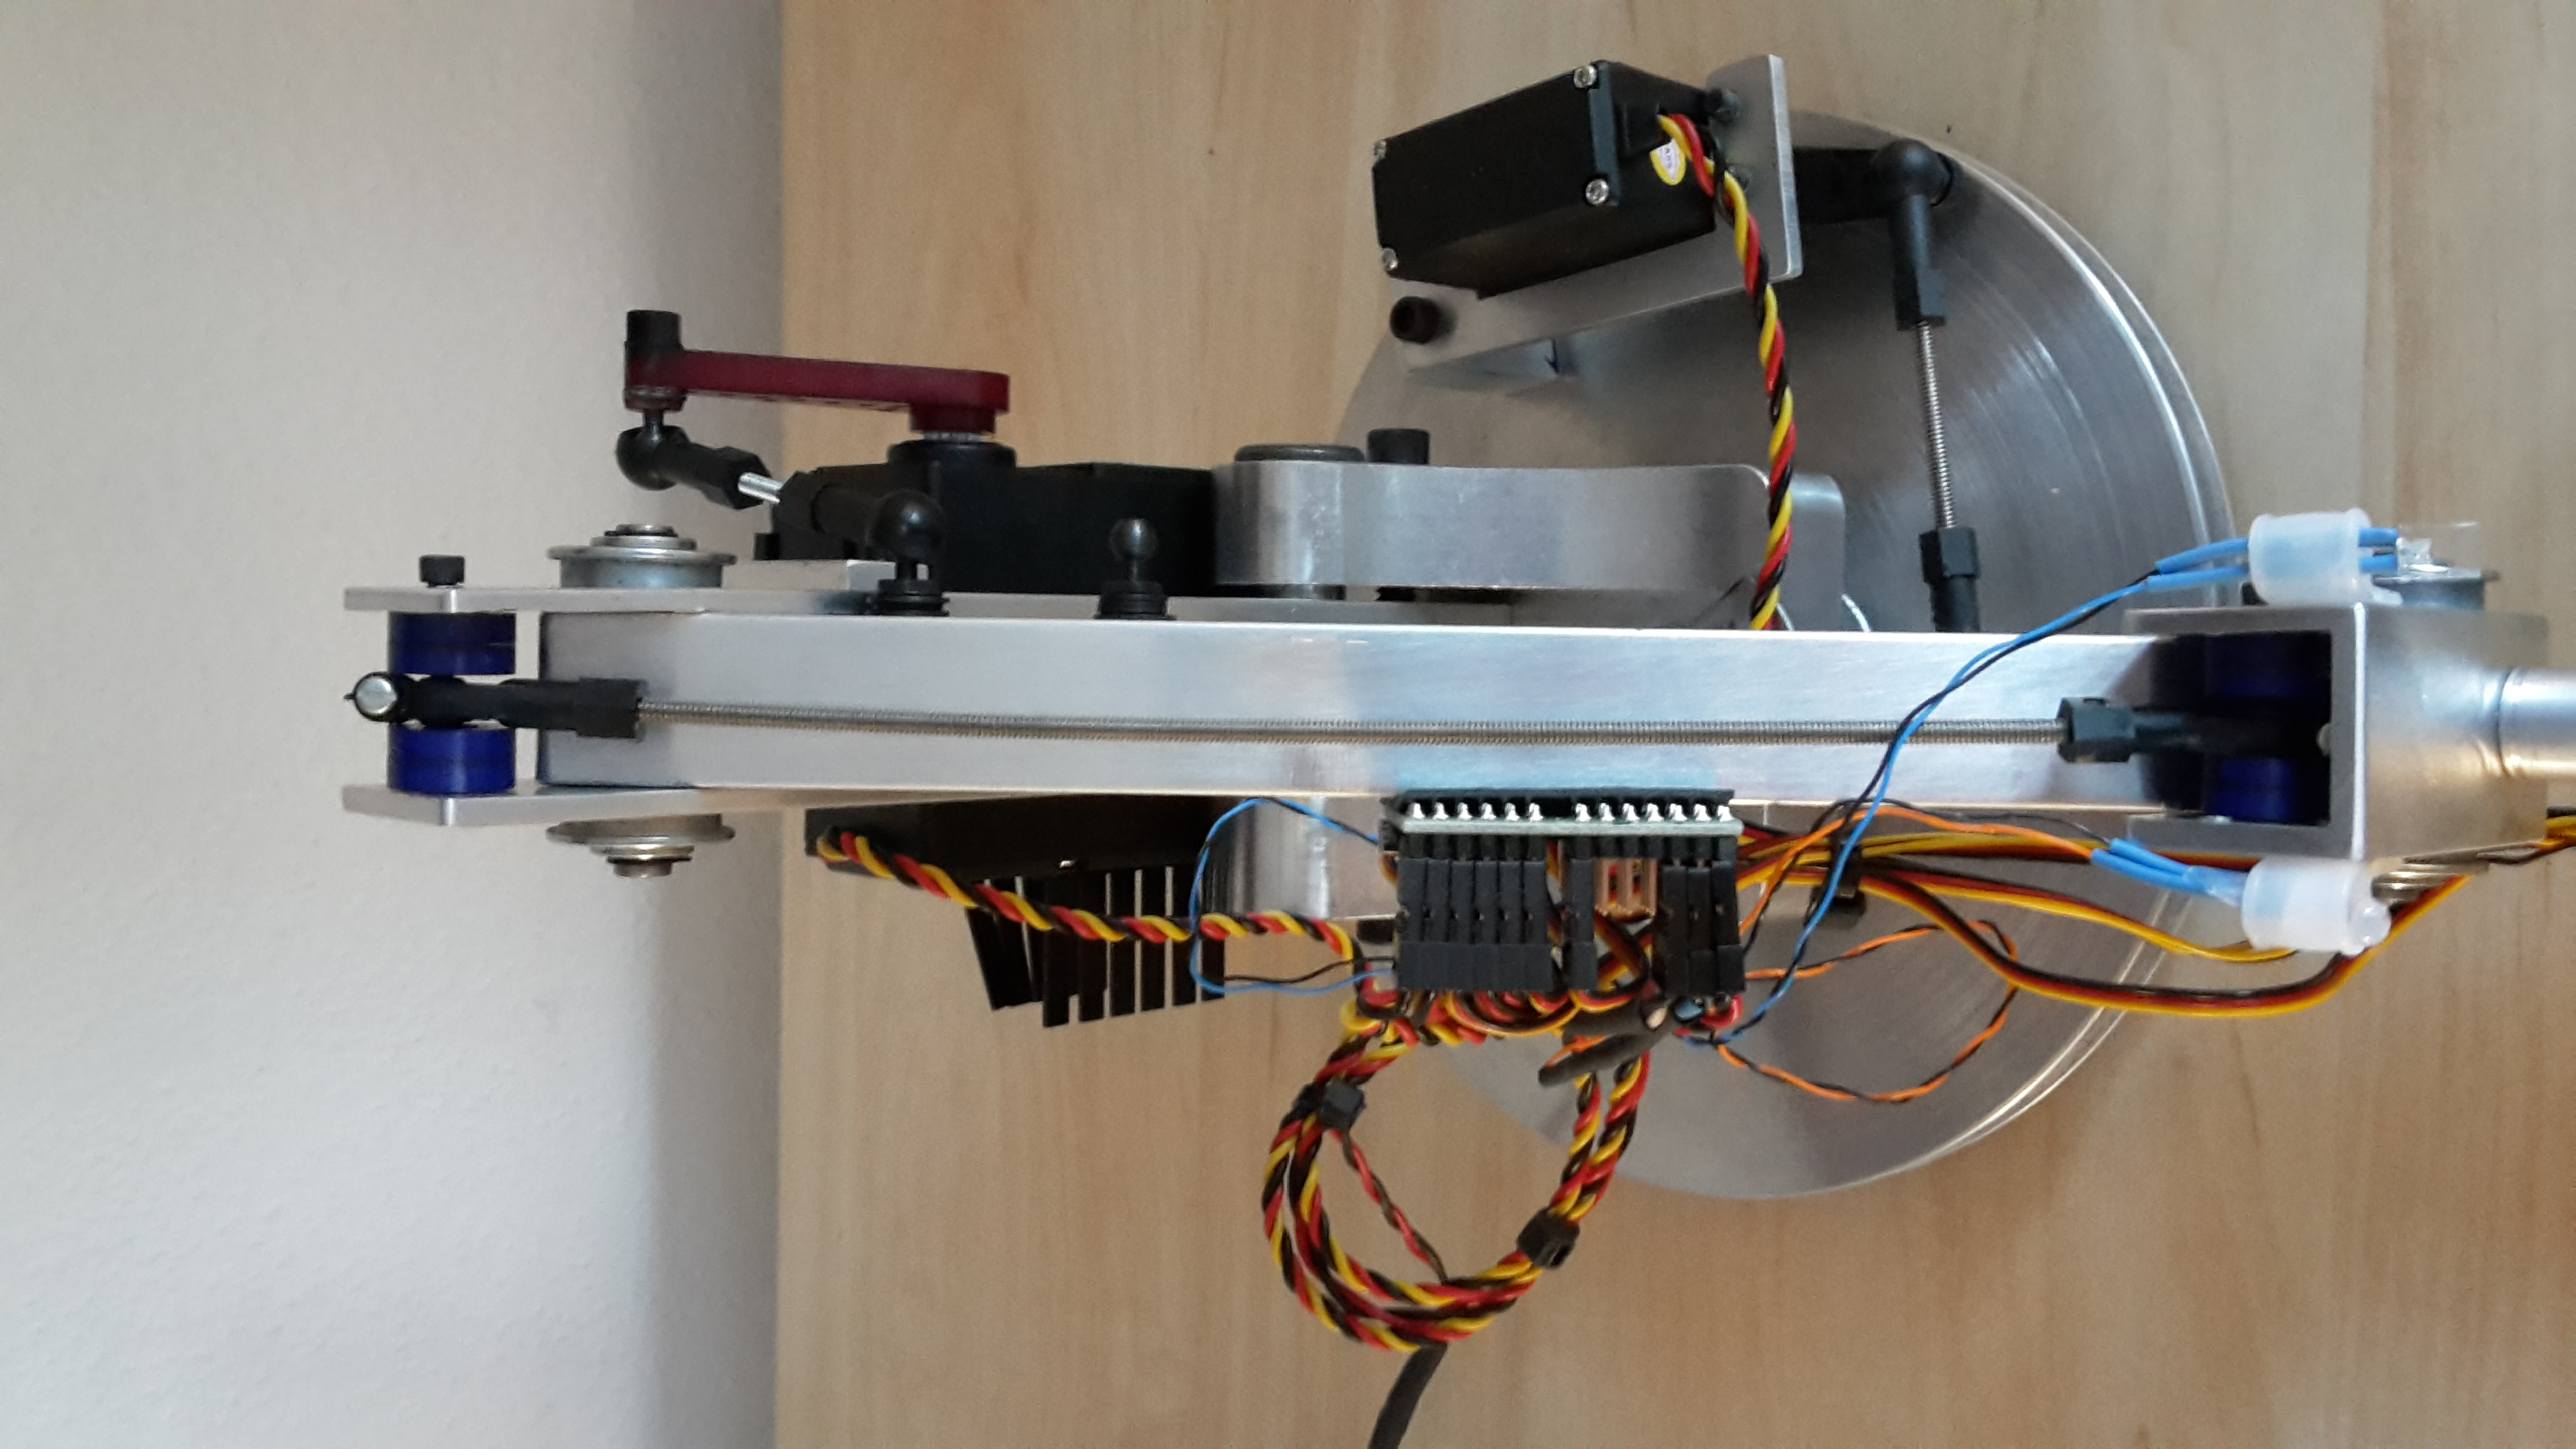
\includegraphics[width=1.1\textwidth, angle=-90]{photos/Day36-pt1.jpg}
	\end{minipage}
	\hfill
	\begin{minipage}{0.455\textwidth}
		\caption{Build Complete}  
		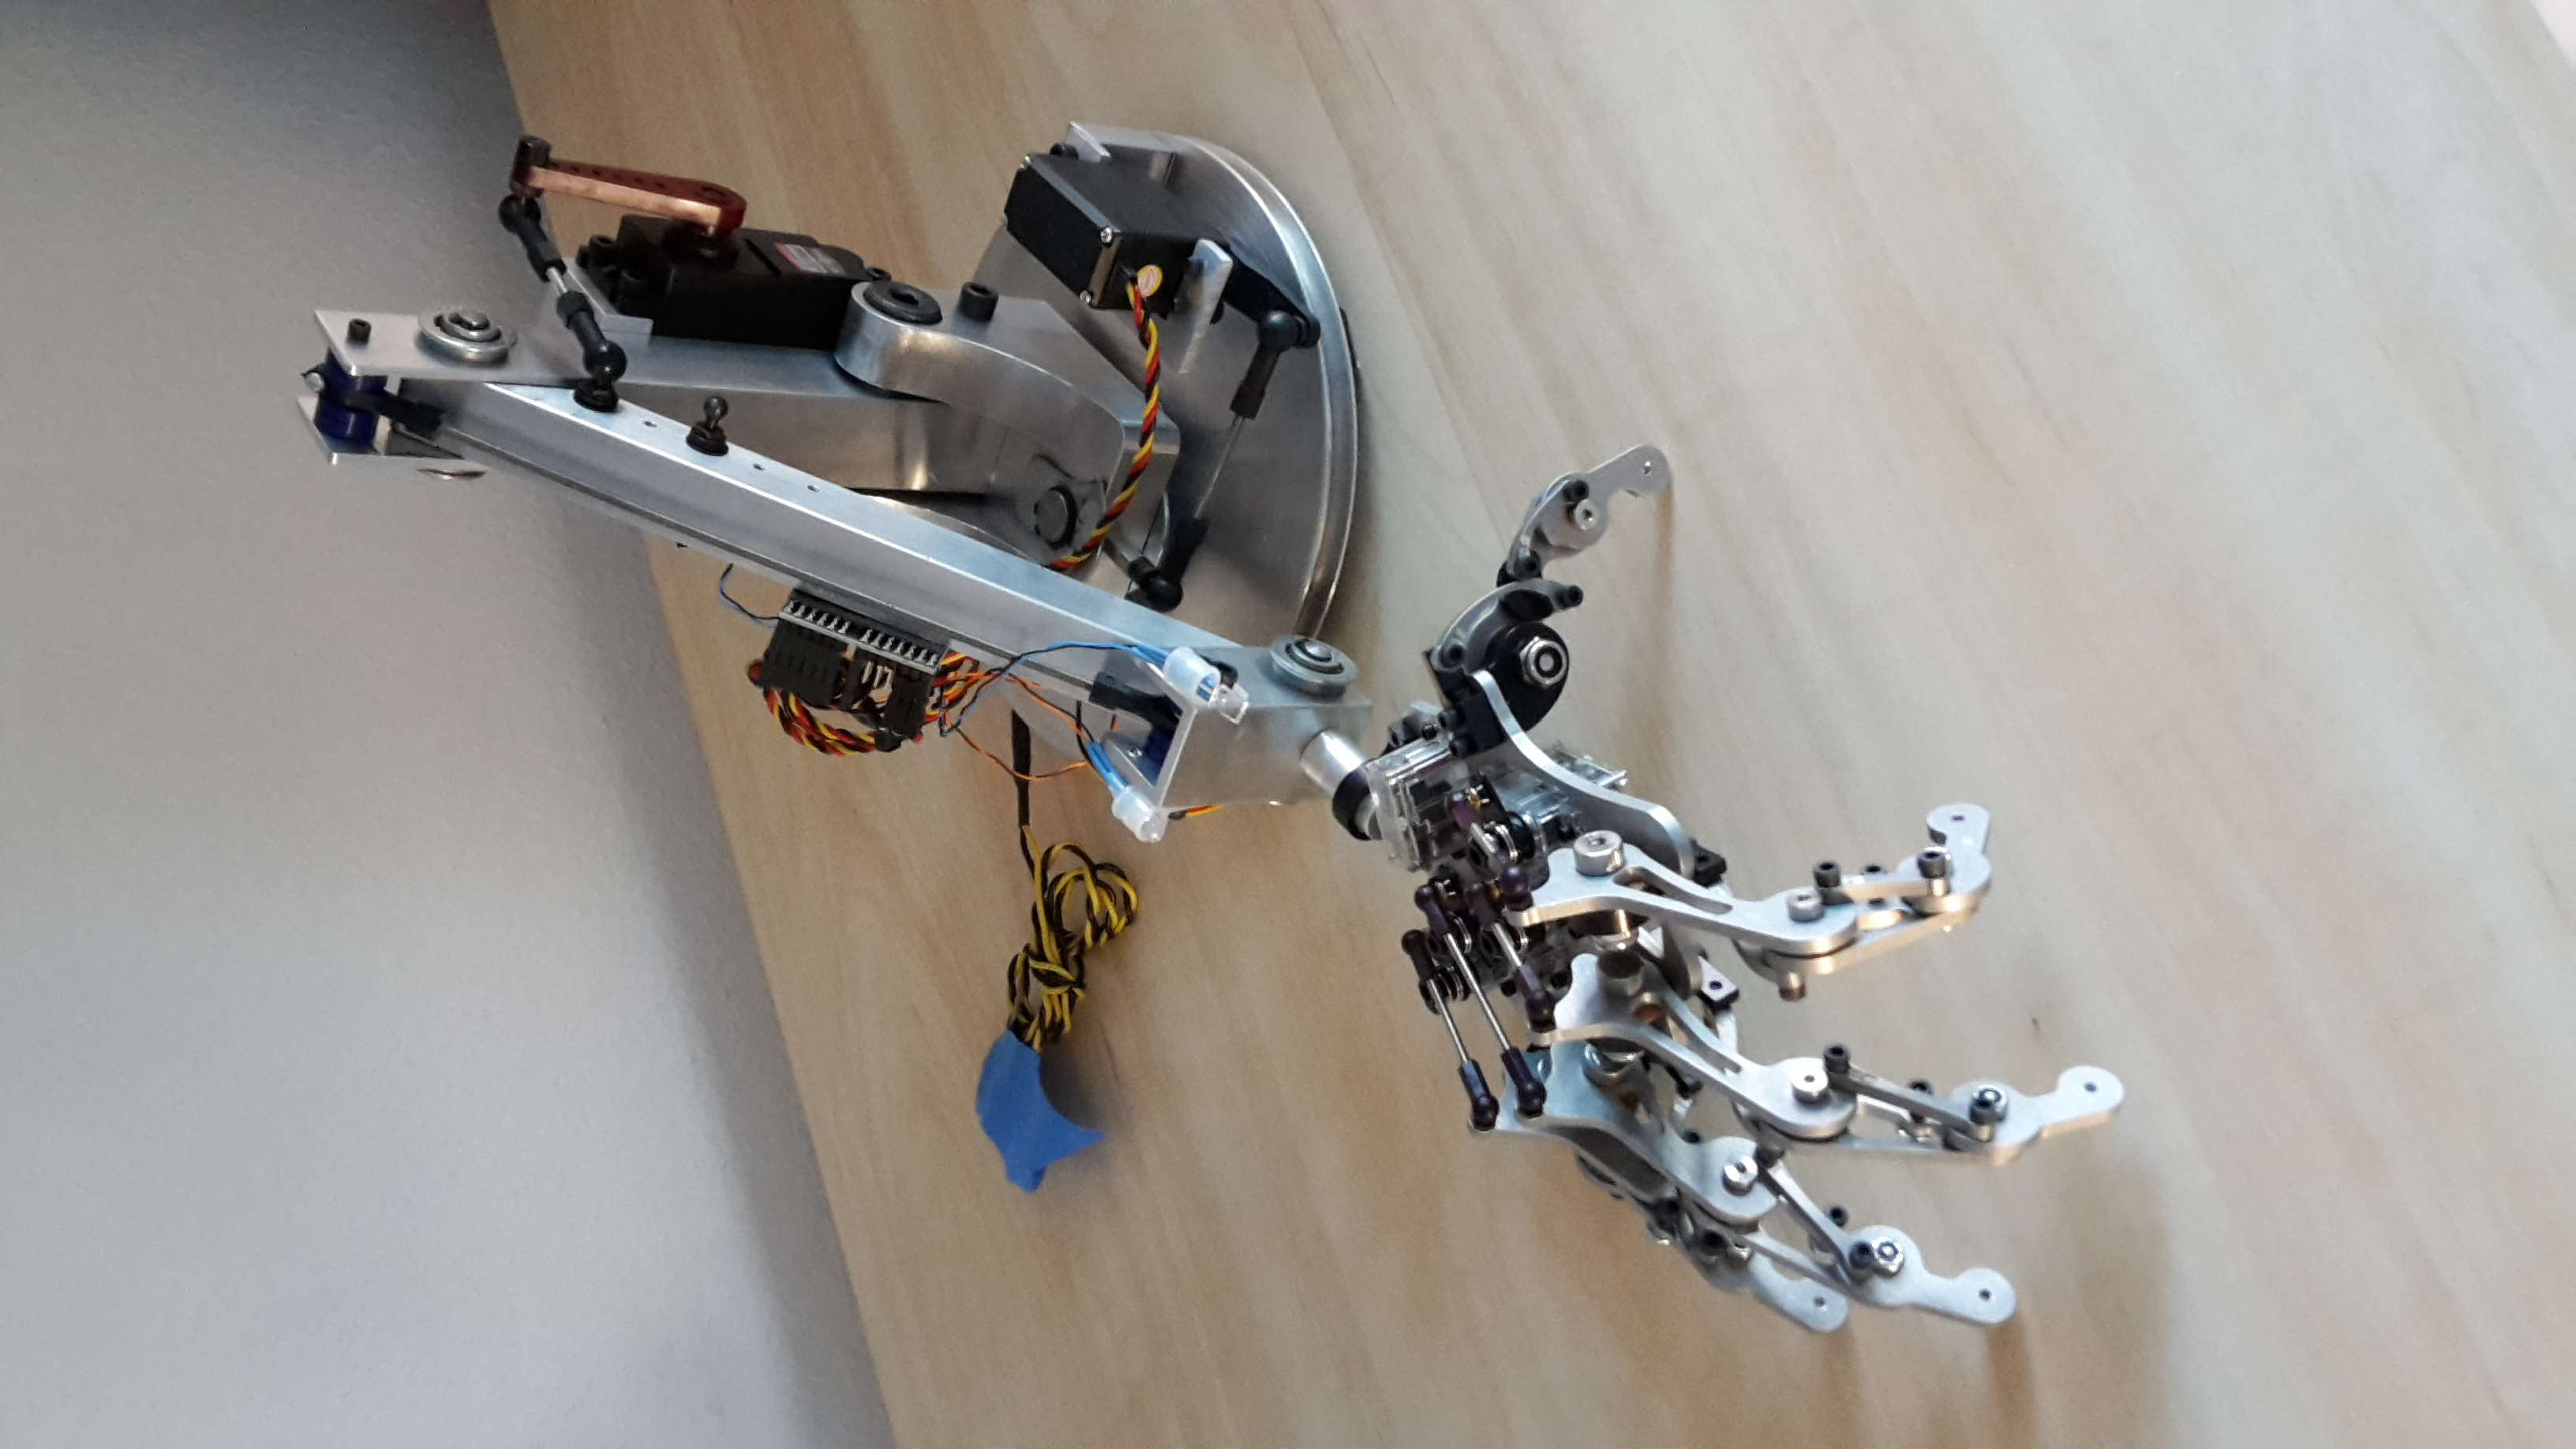
\includegraphics[width=1.1\textwidth, angle=-90]{photos/Day42-pt5.jpg}
	\end{minipage}
\end{figure}

The build does not go completely to plan, as the author originally estimates it will take three full weeks, however it ends up taking over seven. The hand and arm are more complex than expected so there are several welding and placement issues, before the parts are fully positioned. 

Also, when testing the basic coding, the original servos are found to be too strong and cause some movement issues, so new ones have to be ordered and re-inserted onto the hardware. 

\section{Issues and Contingencies}
There are two main issues, so far. The first is the hardware build and basic coding taking longer, and being more complicated, than originally expected. Some of the parts arrive late and, as stated above, some have to be re-ordered and re-inserted onto the hardware. This is entirely caused by mistakes made by the author, due to lack of skills and knowledge. 

The build, however, is fully completed half way through Semester 1 and the basic coding script is written and tested. The hand can currently move up, down, left, right, hold a paper coffee cup, move it and put it down. 

This means the \textbf{\textit{Must Have}} section of the \textit{MoSCoW Analysis} is fully completed and tested, leaving the more complex tracking coding (\textbf{\textit{Should Have}} section) ready to be started. 

The second issue is due to a personal family bereavement, so the project has to be placed on hold for several weeks, causing an unexpected delay. Due to this the author has identified a few potential issues going forward into the next stage of development. They are:
\begin{itemize}		
	\item \textit{Bereavement continuing to impact productivity and efficiency}
	\item \textit{Investigation of complex coding taking longer than expected}
	\item \textit{Hardware breakdowns}
	\item \textit{Combining complex coding with the basic coding script already written}
\end{itemize}
These are considered carefully, along with the current delays, so contingencies can be put in place. 

At the end of this report are two project Gantt Charts. The first (figure 11) shows the original version included in the Project Proposal. This plan needs to change in order to compensate for the delays mentioned above. 

The Christmas holidays are originally unused so, from a contingency viewpoint, this holiday is now included in the revised plan. The remaining tasks are also changed to show new time-lines. These changes will ensure the project remains on target and takes into account the first two potential issues identified above. See second Gantt chart (figure 12) for the revised plan. 

Any potential hardware breakdowns are covered by the author ordering spare backup parts (eg sensors, servos etc) so they can be used immediately, should a breakdown occur. 

This just leaves the last potential issue. Following a few false starts, with trying to add the complex coding to the basic script, the author  decides to write the complex code separately, so no interaction will occur. A decision will be made, at the end of development, as to whether this will be integrated into the basic coding script, or left as a separate process.


\section{Evaluation}
Following careful reflection and evaluation the author feels that, even with the unexpected delays, good progress is being achieved. 

The skill level of the author, for electronics and understanding how software code interacts with hardware, is increasing considerably and all mistakes are being learnt from and will not happen again.

The Design Document, also, turns out to be more important than originally expected. It not only ensures the hardware is built to cover all movement in a human hand but, also, identifies the build as quite complex. 

To mitigate the complexity, the build is started during the summer holidays. If this were left until the start of Semester 1 the unexpected delays will have fallen during the \textit{Must Have} stage, instead of the \textit{Should have} one. This will have made it nearly impossible to recover from however, falling as it does, means the delay will cost the project some time over the Christmas holidays, but it is still possible to catch up.

To ensure no further delays occur, and any potential issues are dealt with quickly and efficiently, progress will continue to be closely monitored during the second half of the project. 

This will be achieved by the author using Trello to keep tasks on target, having regular meetings with their project supervisor and careful project management of their time during Semester 2.

To summarise: the first stage of development is completed and, with the above plan revisions, the project should be completed on time and provide all the requirements needed for a successful delivery.

   \begin{cmpfigure}{Original Project Gantt chart time-table\label{pplan}}
 	\centering
 	\begin{sideways}
 		\newganttchartelement{voidbar}{voidbar/.style={draw=black, top color=black!25, bottom color=black!23}}
 		
 		\begin{ganttchart}[x unit=0.45cm, vgrid, title label font=\scriptsize,canvas/.style={draw=black, dotted}]{1}{34}
 			\gantttitle{Project schedule shown for e-vision week numbers and semester week numbers}{34} \\
 			\gantttitlelist{8,...,41}{1}\\
 			\gantttitlelist{1,...,12}{1}
 			\gantttitle{Christmas}{4}
 			\gantttitlelist{1,...,9}{1}
 			\gantttitle{Easter}{4}
 			\gantttitlelist{10,...,14}{1}\\
 			
 			% Numbered in order of declaration, zero based
 			
 			\ganttbar{Project proposal}{1}{3} \\ %elem0
 			\ganttbar{Literature review}{2}{5} \\ %elem1
 			\ganttbar{Complete design and build}{2}{4} \\ %element 2
 			\ganttbar{Basic coding and testing}{4}{8}\\ %element3
 			\ganttmilestone{Basic code delivery}{9} \\ 
 			\ganttbar{Investigate Tracking}{9}{10}\\ %element 5
 			
 			\ganttbar{Tracking coding}{10}{12} %element 6 & don't include \\ to keep on same line
 			\ganttvoidbar{}{13}{16}  %don't include \\ to keep on same line
 			\ganttbar{}{17}{21}\\
 			
 			\ganttbar{Test Tracking code}{17}{22}\\
 			
 			\ganttbar{Review and Evaluation}{21}{25} \\
 			\ganttmilestone{Completed code delivery}{25} \\  
 			\ganttbar{Final report writing}{23}{30} \\  %work on writing over Easter
 			\ganttbar{Inspection preparation}{31}{34}
 			
 			\ganttlink{elem0}{elem2}
 			\ganttlink{elem1}{elem2}
 			\ganttlink{elem2}{elem3}
 			\ganttlink{elem3}{elem4}
 			\ganttlink{elem4}{elem5}
 			\ganttlink{elem5}{elem6}
 			%elem 6-7 not needed as void   
 			\ganttlink{elem8}{elem9}
 			\ganttlink{elem9}{elem10}
 			\ganttlink{elem10}{elem12}
 			\ganttlink{elem11}{elem13}
 			
 		\end{ganttchart}
 	\end{sideways}
 \end{cmpfigure}

 \begin{cmpfigure}{Revised Project Gantt chart time-table\label{pplan}}
 	\centering
 	\begin{sideways}
 		\newganttchartelement{voidbar}{voidbar/.style={draw=black, top color=black!25, bottom color=black!23}}
 		
 		\begin{ganttchart}[x unit=0.45cm, vgrid, title label font=\scriptsize,canvas/.style={draw=black, dotted}]{1}{34}
 			\gantttitle{Project schedule shown for e-vision week numbers and semester week numbers}{34} \\
 			\gantttitlelist{8,...,41}{1}\\
 			\gantttitlelist{1,...,12}{1}
 			\gantttitle{Christmas}{4}
 			\gantttitlelist{1,...,9}{1}
 			\gantttitle{Easter}{4}
 			\gantttitlelist{10,...,14}{1}\\
 			
 			% Numbered in order of declaration, zero based
 			
 			\ganttbar{Project proposal}{1}{3} \\ %elem0
 			\ganttbar{Literature review}{2}{5} \\ %elem1
 			\ganttbar{Complete design and build}{2}{4} \\ %element 2
 			\ganttbar{Basic coding and testing}{4}{8}\\ %element3
 			\ganttmilestone{Basic code delivery}{9} \\ 
 			\ganttbar{Investigate Tracking}{13}{15}\\ %element 5
 			\ganttbar{Tracking coding}{15}{23} %element 6 work over Christmas
 			\ganttbar{}{24}{24}\\  
 			\ganttbar{Test Tracking code}{20}{25}\\
 			\ganttbar{Review and Evaluation}{22}{27} \\
 			\ganttmilestone{Completed code delivery}{26} \\  
 			\ganttbar{Final report writing}{25}{30} \\  %work on writing over Easter
 			\ganttbar{Inspection preparation}{31}{34}
 			
 			\ganttlink{elem0}{elem2}
 			\ganttlink{elem1}{elem2}
 			\ganttlink{elem2}{elem3}
 			\ganttlink{elem3}{elem4}
 			\ganttlink{elem4}{elem5}
 			\ganttlink{elem5}{elem6}
 			\ganttlink{elem7}{elem8}   
 			\ganttlink{elem8}{elem9}
 			\ganttlink{elem9}{elem10}
 			\ganttlink{elem10}{elem11}
 			\ganttlink{elem10}{elem12}
 			\ganttlink{elem11}{elem13}
 			
 		\end{ganttchart}
 	\end{sideways}
 \end{cmpfigure}

  %bibliographystyle{plainyr-rev}  %shows names and dates
\pagebreak
\bibliographystyle{apalike}  %shows numbers that relate to the citations instead of names and dates
\bibliography{progress}

\end{document}
